\chapter{Koncepcja realizacji}

W niniejszym rozdziale zostanie przedstawiona koncepcja realizacji projektu.

\section{Plan projektu}

Projekt składa się z serwera oraz klienta (aplikacji graficznej komunikatora). Klienci łącząc
się do serwera będą podawać swoją nazwę i będą "wpuszczani" jeżeli do serwera nie jest już
podłączony klient z taką samą nazwą.

Serwer pełni dwie funkcje:

\begin{itemize}
      \item odkrywanie - pozwala połączonym klientom ogłosić swoją dostępność w celu otrzymywania
            połączeń. W tym celu serwer wysyła wszystkim połączonym klientom pełną listę innych
            połączonych klientów za każdym razem gdy ulegnie ona zmianie (czyli np. jeżeli połączy
            się nowy klient lub dowolny z połączonych klientów rozłączy się).
      \item sygnalizacja - aby utworzyć połączenie peer-to-peer pomiędzy klientami, niezbędna jest
            między nimi wymiana informacji przez jakiś inny kanał. W tym celu serwer pośredniczy w
            wymianie wiadomości pomiędzy klientami.
\end{itemize}

Celem klienta jest połączenie z serwerem, a następnie jednoczesne nasłuchiwanie i reagowania na
wiadomości od serwera, a także reagowanie na zdarzenia pochodzące od użytkownika. Gdy ustanawiane
jest połączenie, klient powinien negocjować parametry połączenia z drugim klientem za pomocą
zapewnionego przez serwer kanału, a następnie nawiązać bezpośrednie połączenie P2P z drugim
klientem.

Interfejs graficzny klienta zostanie wykonany we frameworku GTK \cite{gui_rust_gtk}.

Na diagramie \ref{fig:client_states} przedstawiono wszystkie możliwe stany w których może znajdować
się klient oraz wiadomości wysłane lub otrzymane które powodują zmianę danego stanu na inny.

\begin{figure}[H]
      \centering
      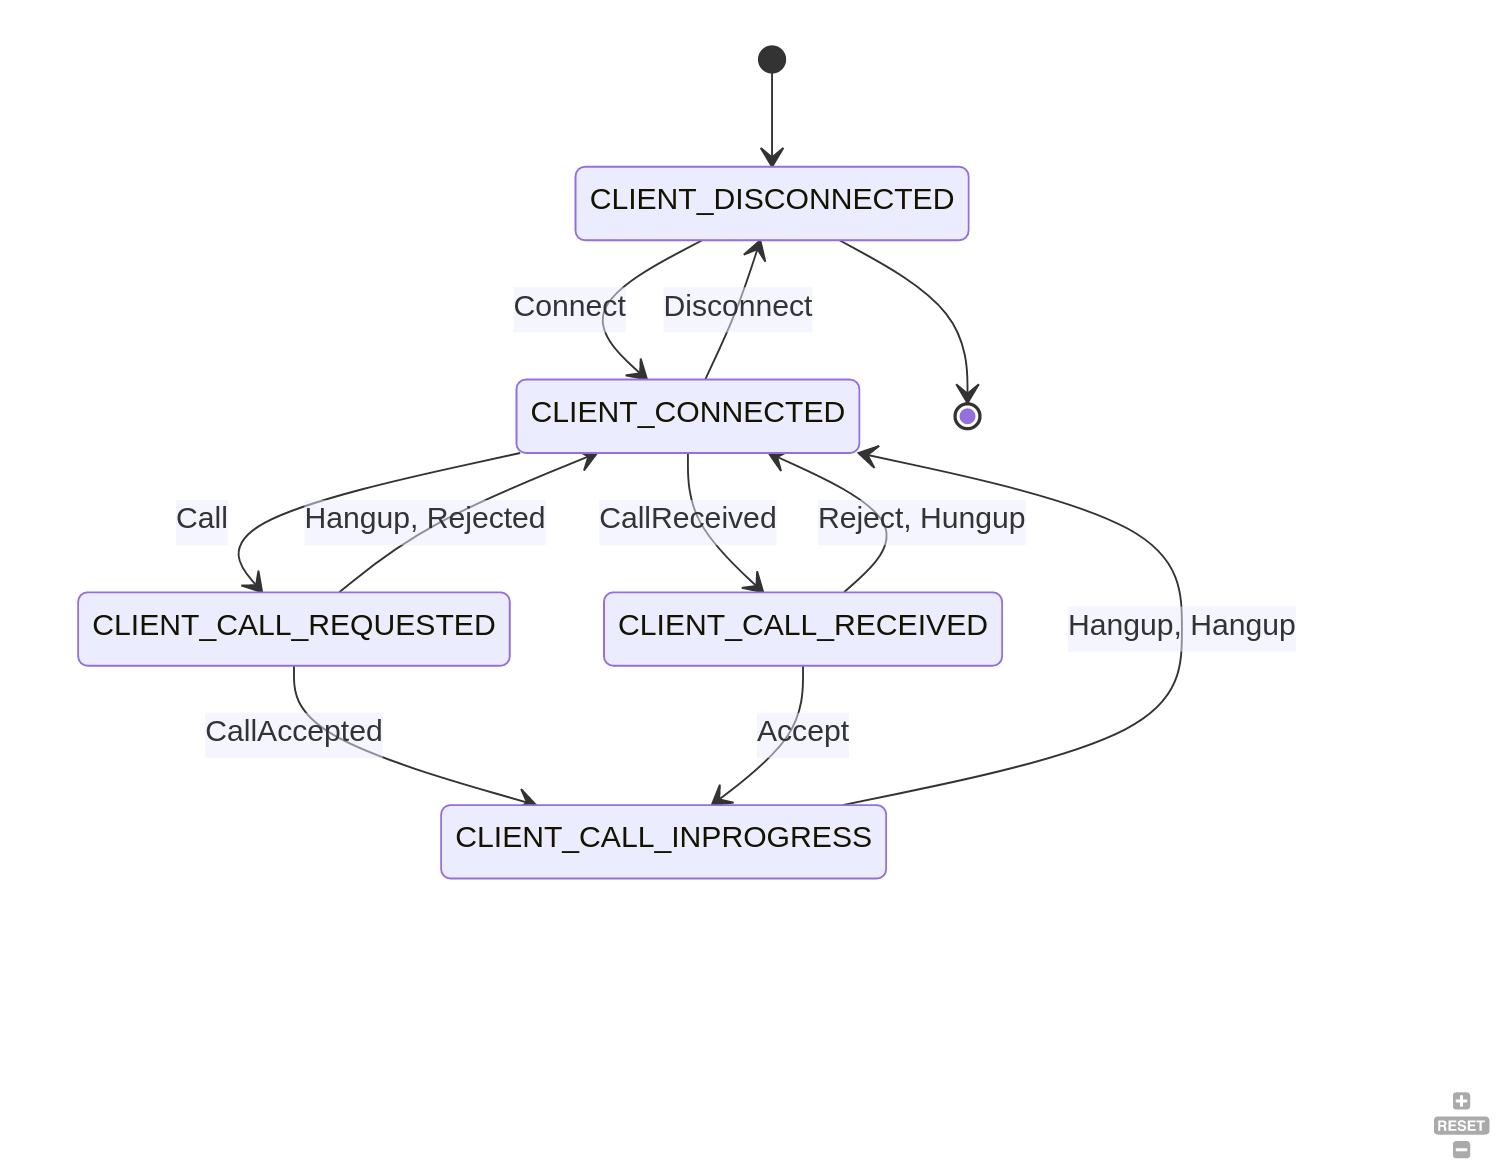
\includegraphics[width=.8\textwidth]{img/rozdzial3/state-diagram-2}
      \caption{Diagram stanów klienta}
      \label{fig:client_states}
\end{figure}

\subsection*{Stany}

\begin{itemize}
      \item \verb|CLIENT_DISCONNECTED| - klient nie jest połączony z serwerem. Klient znajduje się w
            tym stanie zaraz po wykonaniu WebSocket handshake, ale przed wysłaniem wiadomości
            \verb|CONNECT|. W tym wypadku klient musi połączyć się wysyłając wiadomość \verb|CONNECT|
            i nie może wykonywać żadnych innych akcji.
      \item \verb|CLIENT_CONNECTED| - klient jest połączony, może rozpocząć nowe połączenie lub
            otrzymywać połączenia.
      \item \verb|CLIENT_CALL_REQUESTED| - klient zadzwonił do innego klienta, może zakończyć rozmowę
            wysyłając \verb|HANGUP| wracając do stanu \verb|CLIENT_CONNECTED| lub poczekać aż drugi
            klient odpowie, i przejść do stanu \verb|CLIENT_CALL_INPROGRESS|.
      \item \verb|CLIENT_CALL_RECEIVED| - klient otrzymał zaproszenie do rozmowy z innym klientem.
            Może zaakceptować wysyłając \verb|ACCEPT|, lub odmówić wysyłając \verb|REJECT|. Nie może
            rozpoczynać połączeń ani otrzymywać innych połączeń dopóki nie odpowie na przychodzące
            połączenie.
      \item \verb|CLIENT_CALL_INPROGRESS| - klienci są w połączeniu, każdy z nich może zakończyć
            rozmowę wysyłając wiadomość \verb|HANGUP|, przywracając obu klientów do stanu
            \verb|CLIENT_CONNECTED|.
\end{itemize}

\subsection*{Wiadomości}

\begin{itemize}
      \item \verb|CONNECT name| - łączy się z serwerem oraz ogłasza dostępność innym klientom pod
            nazwą \verb|name|. Serwer odsyła \verb|CONNECT_OK| lub \verb|CONNECT_ERR| z powodem dla
            którego nie można się połączyć.
      \item \verb|CALL name| - wysyła zaproszenie do rozmowy klientowi pod nazwą \verb|name|.
      \item \verb|ACCEPT| - akceptuje połączenie przychodzące.
      \item \verb|REJECT| - odrzuca połączenie przychodzące.
      \item \verb|HANGUP| - kończy aktualne połączenie.
      \item \verb|USERLIST userlist| - w stanie \verb|CLIENT_CONNECTED| klient od razu po wejściu w
            ten stan, a także w dowolnym czasie może otrzymać wiadomość \verb|USERLIST| zawierającą
            listę aktualnie dostępnych klientów. Jeżeli klient nie jest w stanie
            \verb|CLIENT_CONNECTED|, to wysłanie tej wiadomości zostanie opóźnione aż klient nie
            będzie w tym stanie.

\end{itemize}

Zarówno wiadomości od klienta (rozpoczęcie połączenia, rozłączenie się) jak i od serwera (pojawił
się nowy użytkownik, otrzymano połączenie) mogą pojawić się w każdym momencie, więc model
komunikacji request/response będzie niewystarczający. Potrzebny jest model komunikacji gdzie każda
ze stron nasłuchuje na przychodzące zdarzenia od drugiej strony połączenia.


